\newcommand{\fakeTheoremOneline}[1]{
  % {\color{\colorTitleApprox}\large \textit{Theorem.}} #1
  #1
}
\newcommand{\fakeTheoremOnelineN}[2]{
  {\color{\colorTitleApprox}\large \textit{Theorem #1.}} #2
}

\newcommand{\thmLine}[3]{${\color{\colorTitleApprox}\large \textit{Theorem #1.}}$ & $#2$ & $\equiv$ & $#3 \cap \fairDecl$}

\begin{frame}{The declarative memory fairness definition is universal}

  \begin{columns}
    
    \begin{column}{0.45\linewidth}
      \begin{center}
        \propSubtrace
      \end{center}    
    \end{column}

    \begin{column}{0.05\linewidth}
      \raisebox{-0.5cm}{\LARGE $\approx$}
    \end{column}
    
    \begin{column}{0.40\linewidth}
      \begin{center}
        \onslide<2->{$\fairDecl \defeq$ \\}
        ${\color{\colorTitleApprox}\underline{prefix\text{-}finite(\lFR)}}$\onslide<2->{
        $\land\ {\color{\colorTitleApprox}\underline{prefix\text{-}finite(\lMO)}}$}
      \end{center}
    \end{column}      

  \end{columns}
  
  \vspace{0.5cm}
  \pause

%   \begin{center}
% {\large     
%     \onslide<3->{
%       % \begin{restatable}{thm}{main}
%       \fakeTheoremOneline{\tsoEquiv} \\
%       % where $M \in \{SC, TSO, RA, StrongCoh\}$.
%       % \end{restatable}      
%     }
%     \onslide<4->{
%       % \mmEquiv{SC}\\ \mmEquiv{RA} \\ \mmEquiv{StrongCOH}
%       \fakeTheoremOneline{\mmEquiv{\SCopfair}{\SCdecl}} \\
%       \fakeTheoremOneline{\mmEquiv{\RAopfair}{\RAdecl}} \\
%       \fakeTheoremOneline{\mmEquiv{\SCOHopfair}{\SCOHdecl}} \\
%     }
%   }
%   \end{center}

  \begin{center}

    \begin{tabular}{r r c l}
      \onslide<3->{\thmLine{1}{\TSOopfair}{\TSOdecl} \\}
      \onslide<4->{
      \thmLine{2}{\SCopfair}{\SCdecl} \\
      \thmLine{3}{\RAopfair}{\RAdecl} \\
      \thmLine{4}{\SCOHopfair}{\SCOHdecl} \\
      }
    \end{tabular}
  
\end{center}
  
\onslide<5->{
    \tikz[overlay,remember picture]{
      \node (Coq) at ([xshift=5.8cm,yshift=-1cm]current page.center){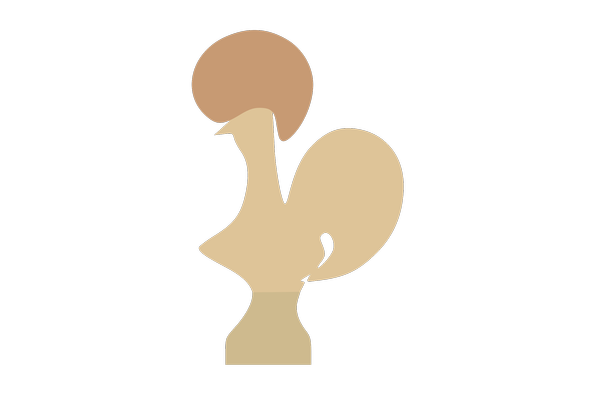
\includegraphics[width=0.3\linewidth]{coq.png}};
  }
  }

\end{frame}


%%% Local Variables:
%%% mode: latex
%%% TeX-master: "oopsla"
%%% End:
